\documentclass[a4paper,12pt]{article}

\usepackage{times}
\usepackage{graphicx}
\usepackage[utf8]{inputenc}
\usepackage[T1]{fontenc}
\usepackage[francais]{babel}
\usepackage{mathtools}
\usepackage{fancyvrb}
\usepackage{url}

\setlength{\parindent}{0in}

\author{David Wong
  \and Jacques Monin
  \and Hugo Bonnin}

\title{Implémentation et Analyse d'une White-box du DES}

\begin{document}

\maketitle

\newpage

\tableofcontents

\newpage

\section{Introduction}

La cryptographie est fondée depuis très longtemps sur ce principe simple : deux personnes veulent pouvoir communiquer entre elles sans pouvoir être écoutées (attaque type Man in the middle).\\
De nombreux block ciphers comme DES ou AES ont été inventés à travers l'histoire de la cryptographie et ont su rester solides contre la cryptanalyse, jusqu'à un certain point.\\

\begin{Verbatim}[samepage=true]
                   MAN IN THE MIDDLE
                           |
       .-----.             |            .-------.
       |     |             v            |       |
       | BOB |   ------------------->   | ALICE |
       |     |                          |       |
       '-----'                          '-------'
\end{Verbatim}

Avec les avancées technologiques des dernières années, de nouveaux besoins en cryptographie ont fait surface. Récemment, le besoin d'exécuter du code contenant des informations sensibles sur des machines potentiellement dangereuses a créé de nouveaux domaines de recherche en Cryptologie.\\

\begin{Verbatim}[samepage=true]
                 .-----------------. 
                 |    ATTAQUANT    |
                 |  .-----------.  |  
                 |  |           |  |  
                 |  |  WHITEBOX |  | 
                 |  |           |  | 
                 |  .-----------.  |
                 |                 |
                 '-----------------'
\end{Verbatim}

\textbf{Man at the end} : l'attaquant a un accès physique au système. Il peut l'inspecter, lui donner les entrées qu'il veut et analyser les sorties, désassembler le logiciel (IDA), voir les appels au système, voir les accès mémoire, émuler des parties du programme... et finalement ce qui nous intéresse : en extraire la clé.\\


\subsection{Utilisation}

Avant d'expliquer une potentielle solution à ce problème, voici quelques illustrations afin de mieux comprendre pourquoi on s'intéresse à cette nouvelle utilisation de la cryptologie :\\


\subsubsection{Backdoors}

Imaginons que le gouvernement français veuille fabriquer un backdoor dormant et infecter diverses machines dans les entreprises/associations/gouvernements de leur choix. Imaginons maintenant qu'il veuille envoyer des instructions à ce backdoor sans qu'elles puissent être interceptées et écoutées, parce que les instructions doivent rester secrètes et/ou parce que l'interception de telles instructions en clair pourrait élever des soupçons.\\

Une des solutions disponibles est d'encrypter ces instructions avec la clé publique/privée de ces backdoors avant de leur envoyer.\\

Personne ne peut lire ces instructions, personne ne peut envoyer d'instructions.

\subsubsection{DRMs}

Imaginons maintenant un système de distribution de film. On encrypte le film avec une clé et on l'envoie avec la clé en annexe. La clé en annexe est elle même encryptée avec la clé de l'utilisateur qui souhaite voir le film. Cette méthode est utilisée pour éviter d'encrypter le film à chaque utilisateur.\\
Le logiciel propriétaire, qui est donc notre fameuse Whitebox, décrypte la clé, décrypte le film ET ajoute un hash de la clé dans le film.\\
L'attaquant peut maintenant soit essayer d'extraire une des deux clés du programme, soit capturer la sortie vidéo pour copier le film. En copiant la sortie vidéo il copiera le hash intégré dans cet output et pourra être incriminé.


\subsubsection{Autres utilisations}

Il existe d'autres utilisations comme les mobile-agents ou les smartcards et sûrement bien d'autres encore qui n'ont pas encore été découvertes...


\subsection{Solution}

C'est là qu'intervient l'idée de la Whitebox. Le but est de rendre l'extraction d'une information importante impossible. Dans notre cas une clé.\\
Barak et cie ont prouvé qu'un obfuscateur parfait n'existait pas dans un article intitulé ``On the (Im)possibility of Obfuscating Programs''\footnote{http://www.iacr.org/archive/crypto2001/21390001.pdf}\\
Cela ne nous empêche pas de nous en approcher. Seulement, peu de théorie a encore vu le jour et les techniques que nous expliqueront par la suite, provenant de l'article de Chow et cie, sont basées sur nos connaissances actuelles des attaques et les observations faites sur la modification des algorithmes de base pour affaiblir ces attaques. Il faut noter que l'état de l'art, sans obfuscation pure, c'est-à-dire en dévoilant les techniques et l'algorithme utilisés, ne fournit pas de solution incrackable actuellement (on trouve la clé en l'ordre de quelques secondes). Ces solutions sont néanmoins utilisées commercialement lorsque les algorithmes et techniques utilisés sont méconnus, et rendent donc la tâche beaucoup plus difficile.\\
Pour finir sur notre explication, une Whitebox est généralement utilisée dans la decryption. Il faut donc, en plus de bloquer l'extraction d'une clé, empêcher l'opération inverse. C'est-à-dire l'encryption. Dans le cas du backdoor, si l'on arrivait à encrypter sans connaître la clé on pourrait alors construire nous même des instructions à destination des backdoors.\\

\newpage
	
\section{Data Encryption Standard}

Avant de nous lancer dans l'implémentation de la version WhiteBox de DES (Data Encryption Standard), nous avons choisi d'implémenter notre propre version de DES afin de nous familiariser avec son fonctionnement (voir notre algorithme sur GitHub : \url{https://github.com/mimoo/DES}).
	
Nous nous intéresserons donc ici au fonctionnement de DES, ainsi qu'à notre approche de son implémentation.

\subsection{Historique et intérêt}

DES est un algorithme de chiffrement symétrique (ou chiffrement par bloc) qui utilise des clés de 56 bits et manipule des blocs de 64 bits. Il a été développé par IBM au début des années 70 à la demande du National Bureau of Standards (NBS) qui proposait de trouver un moyen de sécuriser des informations sensibles, non classifiées, du gouvernement. En 1976, après consultation de la National Security Agency (NSA), le NBS en sélectionne une version légèrement modifiée, qui sera publiée l'année suivante (le standard arrivant en 1979).

Bien qu'il soit recommandé de ne plus l'utiliser (la dernière version avant l'obsolescence datant de 1999), on peut encore parfois le trouver sous la forme de Triple DES.
	
L'intérêt principal d'utiliser DES dans un contexte de type WhiteBox est que cet algorithme a seulement besoin de transformations linéaires et de substitutions, ce qui facilite l'étude du principe. De plus l'algorithme de Triple DES étant encore parfois utilisé, il peut être intéressant de savoir en implémenter une version WhiteBox.

\subsection{Génération des 16 clés}	
	
La clé initiale est représentée sur 64 bits (à laquelle on retire 1 bit de parité à chaque octet). 

Un algorithme est utilisé afin de générer les 16 clés (correspondant aux 16 itérations de DES) issues de la clé initiale. 
	
On commence par retirer les 8 bits de parité de la clé (1 bit à chaque octet). La clé obtenue fait alors 56 bits.
\begin{enumerate}
\item Permutation PC1 puis séparation en deux blocs (droite et gauche).
\item Rotation de chaque bloc vers la gauche (le bit en première position passe en dernière position).
\item Fusion des deux blocs
\item Permutation PC2 de 56 bits vers 48 bits qui correspond à la clé du même numéro que l'itération actuelle. On réutilise le bloc de 56 bits (d'avant la permutation PC2) pour la prochaine itération.
\end{enumerate}

Après ces étapes le bloc est enfin chiffré. Pour déchiffrer ce dernier, on utilise le même algorithme, à ceci près que l'on change l'ordre d'utilisation des clés et que l'on inverse les deux blocs de gauche et de droite au début et à la fin de DES.

\begin{figure}[h]
\centering
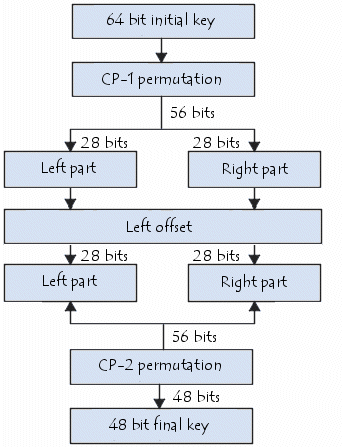
\includegraphics[scale=0.80]{./images/keygen.png}
\caption{Schéma d'une itération de génération de clé}
\label{fig:keygen}
\end{figure}

\clearpage

\subsection{Fonctionnement de DES}	

L'algorithme de DES peut se décomposer en 3 grandes étapes :

\begin{enumerate}
\item Une permutation initiale sur le bloc qui est ensuite divisé en deux blocs de 32 bits.

\item S'ensuit un cycle de 16 itérations effectuant les opérations suivantes :
\begin{itemize}
\item Expansion du bloc de droite de 32 bits vers 48 bits (on copie 16 bits du bloc initial, le tout à l'aide d'un table d'expansion). 
\item XOR entre le nouveau bloc de 48 bits et la clé correspondant au numéro d'itération actuelle.
\item Le bloc de 48 bits est divisé en 8 blocs de 6 bits. Chacun de ces sous-blocs passe à travers une table de substitution (qui prend 6 bits en input et donne 4 bits en output). Il y a en tout 8 tables de substitution, une pour chaque sous-bloc. La valeur en binaire des 4 bits du milieu détermine l'indice de colonne de la table et la valeur binaire des 2 bits extérieurs l'indice de ligne. Le bloc obtenu en fusionnant les 8 sorties de 4 bits a alors une taille de 32 bits.
\item Permutation sur ce bloc (les bits sont changés de place).
\item XOR entre ce bloc et le bloc de gauche.
\item Les deux blocs sont échangés (le bloc de gauche devient celui de droite et inversement).
\end{itemize}


\item Enfin, une fusion des deux blocs, suivie d'une permutation finale, inverse de la permutation initiale.
\end{enumerate}

\begin{figure}[h]
\centering
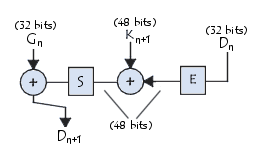
\includegraphics[scale=0.80]{./images/DES_round.png}
\caption{Schéma d'une itération de DES}
\label{fig:DES-round}
\end{figure}

\clearpage

\begin{figure}[h]
\centering
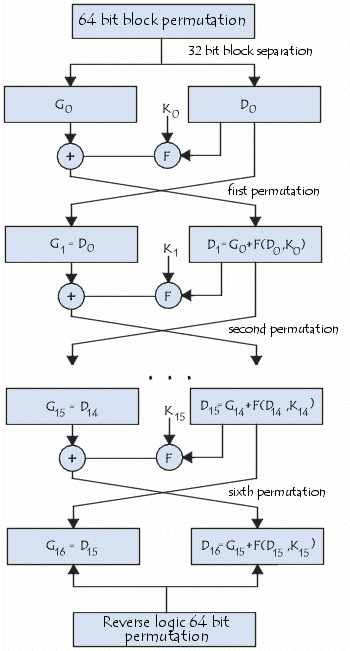
\includegraphics[scale=0.80]{./images/DES_diagram.png}
\caption{Schéma général de DES}
\label{fig:DES-diagram}
\end{figure}

\clearpage

\section{Principes et concepts fondamentaux}

Les Whitebox, telles que définies actuellement, sont des Blackbox destinées à la décryption, à l'intérieur desquelles les clés sont cachées et le processus est assez complexe pour empêcher son inversion.\\
Plusieurs concepts ont été introduits par Chow et cie dans leur article\footnote{http://crypto.stanford.edu/DRM2002/whitebox.pdf}. Voici les trois principaux concepts :


\subsection{Partial Evaluation}

L'évaluation partielle consiste à pré-calculer ce que l'on connaît déjà puis à \textbf{mélanger l'opération du XOR} de la clé avec une autre opération, dans le cas de DES on mélange cette opération avec les substitutions après le XOR.\\
Dans DES, 16 sous-clés sont générées à partir de la clé principale puis sont XORées une à une durant les 16 itérations de l'algorithme. Ces 16 clés de 48bits et les différents résultats de leurs XORs, puis de leurs substitutions avec les $2^{48}$ différents vecteurs possibles à chaque itération sont pré-générés et stockés dans des S-box (Substitution boxes) qu'on appellera \textbf{Lookup tables} par la suite.


\subsection{Tabularizing}

La tabularisation consiste à transformer toutes les autres opérations en \textbf{Lookup tables}.

\begin{verbatim}
  Entrée                 S-box              Sortie
               .----------------------.
0010 := 2 -->  | 0 | 1 | 2 | ... | 15 |
               |----------------------|
               | 5 | 2 | 0 | ... |  8 | --> 0 := 0000
               '----------------------'
\end{verbatim}


\subsection{Input/Output Encoding}

Une fois que toutes les opérations ont été transformées en Lookup tables, il est encore facile de retrouver les opérations initiales et donc d'en extraire la clé. Une façon de rendre ce travail trop fastidieux pour un attaquant est de délinéariser ces opérations en encodant les entrées et sorties de ces Lookup tables.\\

Soit $L_1$ et $L_2$ deux Lookup tables se suivant :\\
$output = L_2(L_1(input))$\\
On peut encrypter la sortie de $L_1$ avec une clé $k_1$ et décrypter l'entrée de $L_2$ avec cette même clé. C'est un \textbf{cipher de Vernam} :\\
On remplace donc $L_1(input)$ par $L_1'(input) = L_1(input) \oplus k_1$\\
et $L_2(input)$ par $L_2'(input) = L_2(input \oplus k_1)$\\
Ce qui donne : $output = L_2'((L_1'(input)))$.\\


\section{Principes et concepts secondaires}

\subsection{Randomization}

Comme l'encryption des entrées/sorties, on peut aussi \textbf{mélanger} les bits sortant d'une opération, puis les remettre dans l'ordre avant la prochaine.\\

Par exemple, si $L_1$ et $L_2$ sont deux lookup tables se suivant :\\
$output = L_2 \circ L_1(input)$\\
 On peut rajouter une bijection $E$ entre les deux comme ceci :\\
$L_2 \circ E^-1 \circ E \circ L_1(input)$


\subsection{Mixing Bijection}

La création des Lookup tables dans la tabularisation se fait à partir de matrices représentant les opérations du cipher. Souvent ces matrices contiennent beaucoup plus de 0 que de 1 ce qui rend les lookup tables trop simples et ce qui crée donc un nouveau problème. Pour éviter ce genre de problème on crée deux opérations au lieu d'une. La première est une bijection. La deuxième est l'inverse de cette bijection multipliéé par l'opération qu'on veut complexifier.\\
Soit $M_1$ la matrice d'une des opérations que l'on transformera en lookup tables plus tard. On peut la multiplier par une autre matrice $G$ choisie de façon pertinente pour augmenter le bruit dans $M_1$ (un nombre de 0 et de 1 qui parait aléatoire). De fait que l'opération devienne alors $G \cdot M_1$. Il faut bien sûr annuler $G$ ensuite en créant une seconde opération $G^{-1}$.\\
L'opération devient alors : $G^{-1} \cdot (G \cdot M_1)$ où $G \cdot M_1$ est pré-évaluée comme une unique opération.


\subsection{By-Pass Encoding}

En général, on veut cacher ce qu'une opération fait. L'idée du bypass est d'élargir la taille de son entrée et la taille de sa sortie avec des bits inutils.


\subsection{Combined Function Encoding}

Lorsque deux opérations sont évaluées en même temps, on peut faire évaluer une entrée composée de leurs deux entrées respectives pour transformer le tout en une seule opération : $(P||Q)(input_P||input_Q)$.

\subsection{Split-Path Encoding}

Lorsque l'on donne un input de n bits, et que l'on reçoit un output de m bits tel que $m < n$ on a une perte d'information. Pour répondre à ce problème on lui concatène une fonction prenant le même input pour augmenter le nombre de bits de sortie.


\subsection{External Encoding}

Pour éviter une extraction de l'implémentation de la whitebox, et pour éviter les attaques sur les premières et dernières itérations, on peut appliquer deux bijections à l'entrée et à la sortie du programme.\\

$Whitebox = E \circ DES(input) \circ G$

\newpage

\section{Implémentation}

Notre implémentation d'une whitebox DES en C est disponible sur notre github : \url{https://github.com/mimoo/whiteboxDES}).\\
Toutes les Lookup tables seront créées par un programme \textbf{Ltablesgen.c} prenant une clé de 64bits en entrée et seront générées dans un fichier qui sera utilisé pour compiler la whitebox plus tard.

\subsection{Bypass et Combined Function Encoding}

\begin{Verbatim}

      **************    **************
      *    L(r)    *    *     R(r)   *
      **************    **************
        |     .------------|  32b
        |     |            v
        |     |  .-------------------.
    32b | 32b |  |       F(R, k)     |
        |     |  '-------------------'
        |     |            |  32b
        v     v            v
       Mem1  Mem2         Mem3
\end{Verbatim}

Ci-dessus la première partie d'une itération de la fonction DES. On peut voir que :

\begin{enumerate}
\item 32bits de la partie gauche restent inchangés pour pouvoir faire un XOR avec la partie de droite encryptée dans la deuxième partie d'une itération.
\item 32 bits de la partie droite subissent des opérations (expansion, xor avec la clé, substitution, permutation).
\item 32 bits de la partie droite restent inchangés pour prendre la place de la partie gauche dans la prochaine itération.
\end{enumerate}

On voit qu'à un moment précis de l'algorithme de DES, la mémoire contient 96 bits. Une analyse de DES plus poussée nous montre facilement qu'il n'existe pas d'état où la mémoire contient plus d'information (en admettant que l'implémentation utilisée soit bien optimisée).\\
Au minimum la mémoire contient 64bits. On va donc garder cet état de 96 bits tout le long et utiliser les bits qui ne servent à rien comme \textbf{bypass}.\\


\subsection{Partial Evaluation}

Les 16 sous-clés sont d'abord pré-évaluées. Puis on pré-évalue l'opération du xor avec la clé, suivi de la substitution que l'on stocke dans des Lookup Tables (différentes à chaque itération puisqu'elles sont influencées par les différentes clés).


\subsection{Tabularisation}

La prochaine étape consiste à transformer toutes les opérations en Lookup tables. Pour ce faire on met d'abord sous forme de matrice chaque opération. Le découpage des opérations sous forme de matrice est expliqué plus loin.\\


\begin{Verbatim}[samepage=true]
       .----.     .-------------------.     .----.
       |    |     |                   |     |    |
       |    |     |                   |     |    |
       |    |     |                   |     |    |
       | Y0 |  =  |         M         |  x  | X0 |
       |    |     |                   |     |    |
       |    |     |                   |     |    |
       |    |     |                   |     |    |
       '----'     '-------------------'     '----'

\end{Verbatim}

Un \textbf{premier problème} survient :\\

Ces matrices contiennent généralement beaucoup trop de zéros (identités, permutations, ...).\\
On utilise d'abord la technique des \textbf{Mixing Bijection} pour séparer la matrice en deux matrices plus complexes (et donc en deux opérations). Mais cela ne suffit pas.\\
Pour éviter d'avoir trop de Lookup tables nulles et réduire le champ de recherche pour l'attaquant, chaque matrice est découpée en \textbf{blocs de sous-matrices}.\\
Les multiplications des sous-matrices aux vecteurs associés sont ensuite transformées en Lookup tables.\\

\begin{Verbatim}[samepage=true]

       .----.     .----.----.----.----.     .----.
       |    |     |    |    |    |    |     | X0 |
       | Y0 |     | A  | B  | C  | D  |     .----|
       |    |     |    |    |    |    |     | X1 |
       .----.  =  .----.----.----.----.  x  .----.
       |    |     |    |    |    |    |     | X2 |
       | Y1 |     | E  | F  | G  | H  |     .----.
       |    |     |    |    |    |    |     | X3 |
       '----'     '----'----'----'----'     '----'
           
\end{Verbatim}

avec Y0 = A*X0 $\oplus$ B*X1 $\oplus$ C*X2 $\oplus$ D*X3

Un \textbf{second problème} survient :\\

On ne peut pas faire des Lookup tables trop grosses car leur taille augmente exponentiellement :\\

Pour 8 bits d'entrée, il y a $2^{8}$ possibilités. Donc la taille de la Lookup table est de $2^{8} * sizeof(output)$.\\
Pour 16 bits d'entrée, il y a $2^{16}$ possibilités. Donc la taille de la Lookup table est de $2^{16} * sizeof(output)$.\\
Avec notre exemple simplifié, en utilisant des Lookup tables prenant 8 bits en entrée, et donc en multipliant par deux le nombre de Lookup tables, on réduit la taille de notre fichier final par $(2^{16} - 2^8 + 2^8) * sizeof(output)$ pour chaque Lookup table.
etc...\\

L'article de Link et cie\footnote{http://eprint.iacr.org/2004/025.pdf} conseille, pour plus de sécurité, de choisir des blocs de 8x4 à la place de 8x8 que conseillent Chow et cie.\\



\begin{figure}[h]
\centering
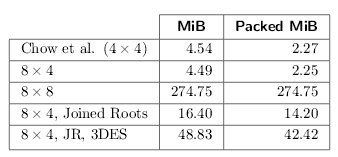
\includegraphics[scale=0.80]{./images/linketal.PNG}
\caption{Différence de taille selon la taille des blocs}
\label{fig:sizedif}
\end{figure}




Chaque sous-matrice va être la source d'une nouvelle lookup table qui sera créée par la multiplication de la sous-matrice avec toutes les possibilités d'input de 4 bits.\\

Ensuite chaque ligne de Lookup table donnera des outputs de 8 bits qu'il faudra XORer entre eux. Pour continuer la tabularisation, chaque XOR est pré-calculé dans ce qu'on appellera des XOR tables.\\

Ce qui donne des \textbf{réseaux} de lookup tables :\\

\begin{Verbatim}[samepage=true]

     ******  ******    ******  ******
     * AX1*  * BX2*    * CX3*  * DX4*
     ******  ******    ******  ******

        |      |          |       |
        v      v          v       v

        8b    8b          8b     8b
      <----><---->      <----><---->
      .----------.      .----------.
       \   S0   /        \   S1   /
        '------'          '------'
         <---->            <---->
           8b                8b

                \         /
                 \       /
                  |     |
                  v     v

                  8b    8b
                <----><---->
                 .---------.
                 \   S2   /
                  '------'
                   <---->
                     8b

                      |
                      v

                   ******
                   * Y0 *
                   ******

\end{Verbatim}

\subsection{Split-Path Encoding}

On a maintenant un réseau de XOR Tables qui prennent 16 bits en input et rendent 8 bits en output. Il y a donc une perte d'information, ce que l'on peut corriger en modifiant ces Look up tables pour avoir un output de 16 bits avec 8 bits de bypass.\\
$L_1'(input) = L_1(input)||R(input)$ avec R une fonction rendant 8 bits en output.
 
\subsection{Input/Output Encoding}

Ce réseau de XOR Tables est maintenant modifié en encryptant/décryptant les entrées-sorties entre opérations. On peut générer des clés de 16 bits en fonction de la clé principale.

\subsection{Matrices}

La suite explique comment les opérations ont été réduites en 3 matrices $M_1$, $M_2$ et $M_3$

\subsubsection{Étape préliminaire}

Avant que les 16 itérations ne s'exécutent, il est nécessaire que les bits d'input subissent une permutation initiale suivie d'une expansion de l'input de 64 bits en 96 bits qui permettra le bypass.
Ces deux opérations seront réalisées par une matrice M1 qui ne sera utilisée qu'une fois juste avant les 16 itérations et qui réalisera ceci :

\begin{Verbatim}[samepage=true]

            96b           96x64b           64b
           .----.     .-------------. 
           |    |     |             |     .----.
           |    |     |             |     |    |
           |    |     |             |     |    |
           |    |     |             |     |    |
           | Y0 |  =  |     M1      |  x  | X0 |
           |    |     |             |     |    |
           |    |     |             |     |    |
           |    |     |             |     |    |
           |    |     |             |     '----'
           '----'     '-------------'

\end{Verbatim}


Nous décomposons M1 en sous-matrices de taille 4x8. Nous multiplions chacune de ces $\frac{96*64}{4*8}$ = 288 sous-matrices par les $2^8$ = 256 différentes possibilités ayant $2^4$ = 16 résultats possibles.


\subsubsection{Étape 1 à étape 2}

Nous devons convertir ce fonctionnement :

\begin{Verbatim}[samepage=true]
			
             32b               48b              16b
           ************** ********************* ********
state 1:   *     L(r)   * *       X(r)        * * r(r) *
           ************** ********************* ********
                 |                |      |         |
                 |                v      |         |
                 | *********    .....    |         v
                 | * sK(r) *--> . + .    |    .-------.
                 | *********    .....    '-->(  Merge  )
                 |                |           '-------'
                 |                v               |
                 |         .-------------.        |
                 |          \     S     /         |
                 |           '---------'          |
                 |                |               |
            32b  v                v 32b     32b   v
           ************** *************** ***************
state 2:   *    L(r)    * *    Y(r+1)   * *     R(r)    *
           ************** *************** ***************

\end{Verbatim}		

En celui-ci :

\begin{Verbatim}[samepage=true]

            *********************************************
state 1:    *          state 1 (12 x 8 = 96 bits)       *
            *********************************************
               |      |      |                       |
               v      v      v                       v
            .-----..-----..-----.                 .-----.
            | T0  || T1  || T2  |       ...       | T11 |
            '-----''-----''-----'                 '-----'
               |      |      |                       |
               v      v      v                       v
            *********************************************
state 2:    *              state 2 (96 bits)            *
            *********************************************			
			
\end{Verbatim}
		
				
Pour ce faire, nous allons calculer 12 Lookup Tables qui prendront 8 bits chacun ce qui recouvrira les 96 bits d'input et qui seront composées de :
\bigskip
\begin{enumerate}
\item 8 lookup tables non linéaires qui permettent le XOR avec la clé et la substitution en les pré-calculant grâce à la formule :

\medskip
\begin{center}
$T_i(x) = S_i(x \oplus k_i)$ 
\end{center}
\medskip

Une permutation est faite sur les données, chaque lookup table non linéaire va donc prendre en paramètre deux bits de L(r-1) et 6 bits de X(r-1) et renverra 2 bits de L(r-1), 2 bits de R(r-1) et 4 bits qui formeront Y(r). Elles sont de la forme :

\begin{Verbatim}[samepage=true]

  L(r-1)                   X(r-1)
.--|--|------------|---|---|---|---|---|-----.
|  |  |            |   |   |   |   |   |     |
|  |  |  .---------o   |   |   |   |   |     |
|  |  |  |         |   |   |   |   |   |     |   
|  |  |  |         |   |   |   |   |   |     |  
|  |  |  |  .------|---|---|---|---|---o     | 
|  |  |  |  |      |   |   |   |   |   |     | 
|  |  |  |  |      |   |   |   |   |   | k(j)|  
|  |  |  |  |      +---+---+---+---+---+-----|  
|  |  |  |  |      |   |   |   |   |   |     | 
|  |  |  |  |      |   |   |   |   |   |     | 
|  |  |  |  |    .-----------------------.   |              
|  |  |  |  |     \                     /    |              
|  |  |  |  |      \        S(j)       /     |              
|  |  |  |  |       \                 /      |               
|  |  |  |  |        '---------------'       |               
|  |  |  |  |          |   |   |   |         |     
|  |  |  |  |          |   |   |   |         | 
|  |  |  |  |          |   |   |   |         |   
'--|--|--|--|----------|---|---|---|---------'
   v  v  v  v          v   v   v   v 
  L(r-1)  R(r-1)            Y(r)

\end{Verbatim}	


L'output de ces lookup tables est donc :
\medskip
\begin{center}
$T_i^r = b_0 b_1||b_2 b_7||S_j(b_2 b_3 b_5 b_6 b_7 \oplus k_i^r)$ 
\end{center}
\medskip

\item 4 lookup tables linéaires qui nous serviront à bypasser les bits qui ne subissent pas de calculs.

Après permutation, les lookup tables linéaires prendront en paramètre 4 bits de la partie gauche de L et 4 bits de la partie des bits non étendus de R. Elles sont sous la forme :

\begin{Verbatim}[samepage=true]
                               _____
          L(r-1)               R(r-1)
.-----|---|---|---|--------|---|---|---|-----.
|     |   |   |   |        |   |   |   |     |
|     |   |   |   |        |   |   |   |     |
|     |   |   |   |        |   |   |   |     |  
|     |   |   |   |        |   |   |   |     | 
|     |   |   |   |        |   |   |   |     |
|     |   |   |   |        |   |   |   |     |
|     |   |   |   |        |   |   |   |     |
|     |   |   |   |        |   |   |   |     | 
|     |   |   |   |        |   |   |   |     | 
|     |   |   |   |        |   |   |   |     | 
|     |   |   |   |        |   |   |   |     |             
|     |   |   |   |        |   |   |   |     |              
|     |   |   |   |        |   |   |   |     |             
|     |   |   |   |        |   |   |   |     |               
|     |   |   |   |        |   |   |   |     |                
|     |   |   |   |        |   |   |   |     |     
|     |   |   |   |        |   |   |   |     | 
|     |   |   |   |        |   |   |   |     |  
'-----|---|---|---|--------|---|---|---|-----'
      v   v   v   v        v   v   v   v 
          L(r-1)               R(r-1)
 
\end{Verbatim}	

L'output de ces lookup tables est donc :
\medskip
\begin{center}
$T_i^r = b_0 b_1 b_2 b_3||b_4 b_5 b_6 b_7$
\end{center}
\medskip
\end{enumerate}



		
\subsubsection{Étape 2 à étape 3}

\begin{Verbatim}[samepage=true]

           ************** *************** ***************
state 2:   *    L(r)    * *    Y(r+1)   * *     R(r)    *
           ************** *************** ***************
                 |                  |           |
                 v                  |           |
               .....    .--------.  |           |
               . + .<---|    P   |<-'           |
               .....    '--------'              |
                |                               |
            32b '----------------------------------.
                                    |           |  |
                .-------------------|-----------'  |
                |               32b v              v 32b
                |               .-------.       .------.
                |              /  E-box  \     ( Select )
                |  32b        '-----------'     '------'
                |                   |              |
                v               48b v              v 16b
           ************** ********************* ********
state 3:   *   L(r+1)   * *       X(r+1)      * *r(r+1)*
           ************** ********************* ********

\end{Verbatim}


Comme pour l'étape précédente, nous voulons transformer les différentes opérations de cette étape en look up tables.

Pour ce faire, nous allons modéliser les différentes opérations en matrices puis la décomposer puisque la combinaison de la permutation et du XOR est une fonction affine.

Ces calculs vont être modélisés par M2 qui est une matrice (96,96) et qui réalise :
\begin{enumerate}
\item La permutation
\item Le xor avec la partie gauche
\item L'expansion pour la prochaine itération
\item Le placement de R(r) dans L(r+1) 
\item L'extraction le vrai R(r).
\end{enumerate}



\subsubsection{Étape finale}

L'étape finale va consister à ignorer les bypass (ie, ignorer r(r+1)), inverser la dernière expansion réalisée par M2, échanger L et R en cas de décryptage et faire la permutation finale.

Toutes ces étapes vont être réalisées grâce à une matrice M3 qui va être décomposée en sous-matrices et traduite en Lookup tables.

\newpage

\section{Conclusion}

L'implémentation d'une whitebox demande une recherche et des efforts considérables. Il faut considérer les autres solutions disponibles (utilisation d'une API, d'une clé publique, ...) avant de commencer à entreprendre la construction d'une whitebox.\\

La taille que prend une whitebox est considérablement plus important que la taille d'un cipher nu. L'implémentation de Chow et al est par exemple de 4.5 MB. Une implémentation hardware est donc peu envisageable.\\

La sécurité des techniques publiées par Chow et cie provient essentiellement de l'encryption des entrées/sorties et de leur nombre. Mais cela ne suffit pas, aucune implémentation de whitebox dont les techniques et les algorithmes sont connus n'est sécurisée à ce jour.\\

Dans le cas où le lecteur serait intéressé par une solution professionnel du type whitebox, ces techniques seront utiles mais certainement non-suffisantes. D'autres sont surement utilisées mais non publiées afin de compliquer les attaques possibles.\\

\newpage

\section{Bibliographie}

``A White-box DES Implementation for DRM Applications'', Chow et cie.\\
\url{http://crypto.stanford.edu/DRM2002/whitebox.pdf}

``White-Box Cryptography'' (PhD thesis), B. Wyseur.\\
\url{https://www.cosic.esat.kuleuven.be/publications/thesis-152.pdf}

``Practical cracking of white-box implementations'', B. Wyseur.\\
\url{http://www.phrack.org/issues.html?issue=68&id=8#article}

``White-Box Cryptography'' (Vidéo), Dmitry Khovratovich.\\
\url{https://www.youtube.com/watch?v=om5AVTqB5bA}

``On the (Im)possibility of Obfuscating Programs'', Barak et cie.\\
\url{http://www.iacr.org/archive/crypto2001/21390001.pdf}

``Clarifying Obfuscation: Improving the Security of White-box Encoding'', Hamilton E. Link and William D. Neumann.\\
\url{http://eprint.iacr.org/2004/025.pdf}


\end{document}
